\documentclass[18 pt]{beamer}
\usetheme{Madrid}
% \usefonttheme{professionalfonts}
\usefonttheme{structurebold}
\usecolortheme{rose}
\setbeamerfont{title}{size=\LARGE, series=\bfseries}
\usepackage{subfigure}
\usepackage{enumitem}

\setlist[enumerate]{label=\indent\indent, leftmargin=*,itemsep=
1pt,parsep = 1pt}
\setbeamerfont{enumerate item}{size=\LARGE}

\usepackage{amsmath}
\usepackage{amssymb}
\usepackage{listings}
\usepackage{booktabs}
\usepackage{multirow}
\usepackage{multirow}
\usepackage{lmodern}
\usepackage{xcolor}
\usepackage{float}
\lstset{
  language=Python,  %代码语言使用的是matlab
  % frame=shadowbox, %把代码用带有阴影的框圈起来
  rulesepcolor=\color{red!20!green!20!blue!20},%代码块边框为淡青色
  keywordstyle=\color{blue!90}\bfseries, %代码关键字的颜色为蓝色,粗体
  commentstyle=\color{red!10!green!70}\textit,    % 设置代码注释的颜色
  basicstyle=\footnotesize,
  showstringspaces=true,%不显示代码字符串中间的空格标记
  % numbers=left, % 显示行号
  % numberstyle=8pt,    % 行号字体
  % numberstyle=\color{green},
  stringstyle=\rmfamily\slshape\color[RGB]{128,0,0}, % 代码字符串的特殊格式
  breaklines=true, %对过长的代码自动换行
  extendedchars=false,  %解决代码跨页时,章节标题,页眉等汉字不显示的问题
  escapeinside=``,%代码中出现中文必须加上,否则报错
  texcl=true}

\lstset{breaklines}%自动将长的代码行换行排版

\lstset{extendedchars=false}%解决代码跨页时,章节标题,页眉等汉字不显示的问题

\usepackage{textcomp}
% \usepackage[margin=1in]{geometry}
\usepackage{pythonhighlight}
% \usepackage{minted}
\usepackage[backend=bibtex]{biblatex}
%\usepackage[style=authortitle,backend=biber]{biblatex}
\addbibresource{ResearchRabbit_Export_2022_10_20.bib}

\usepackage{algorithm}
\usepackage{algorithmic}
\renewcommand{\algorithmicrequire}{\textbf{Input:}}
\renewcommand{\algorithmicensure}{\textbf{Output:}}

\AtBeginSection[]{
  \begin{frame}
  \frametitle{Outline}
  \tableofcontents[currentsection]
  \end{frame}
}
\setbeamertemplate{section in toc}{\inserttocsectionnumber.~\inserttocsection}
\setbeamertemplate{subsection in toc}[ball unnumbered]
\setbeamertemplate{subsubsection in toc}[square unnumbered]


\title{Modular Software for Real-Time Quantum Control Systems}
\author[Gcc]{Dingchao Gao}
\institute[ISCAS]{Institute of Software Chinese Academy of Sciences}

\setbeamertemplate{footline}[frame number]
\begin{document}

\frame{\titlepage}

\begin{frame}{Overview}
  \begin{figure}
    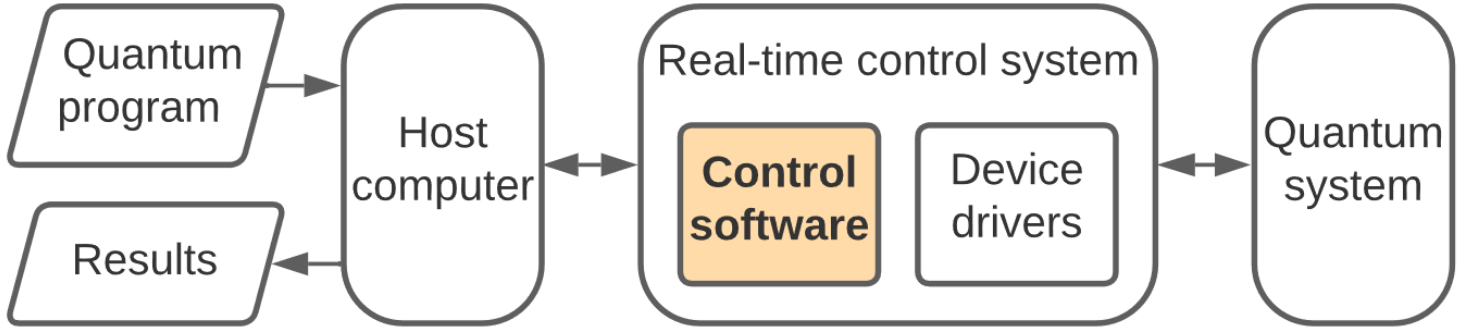
\includegraphics[width=.8\textwidth]{real-time.png}
  \end{figure}
\end{frame}
\begin{frame}{Overview}
\begin{itemize}
\item Presents modular software architecture for quantum control systems
\item Goals: Flexibility, portability, performance
\item Introduces Duke ARTIQ Extensions (DAX) framework
\end{itemize}
\end{frame}

\begin{frame}{Modular Software Architecture}
\begin{itemize}
\item Modules - group devices with tight control needs
\item Services - system-wide functions using modules
\item Registry - central catalog of modules and services
\item Interfaces - standard functionality descriptions
\item Clients - portable code using interfaces
\end{itemize}
\end{frame}
\begin{frame}{Modular Software Architecture}
  \begin{figure}
    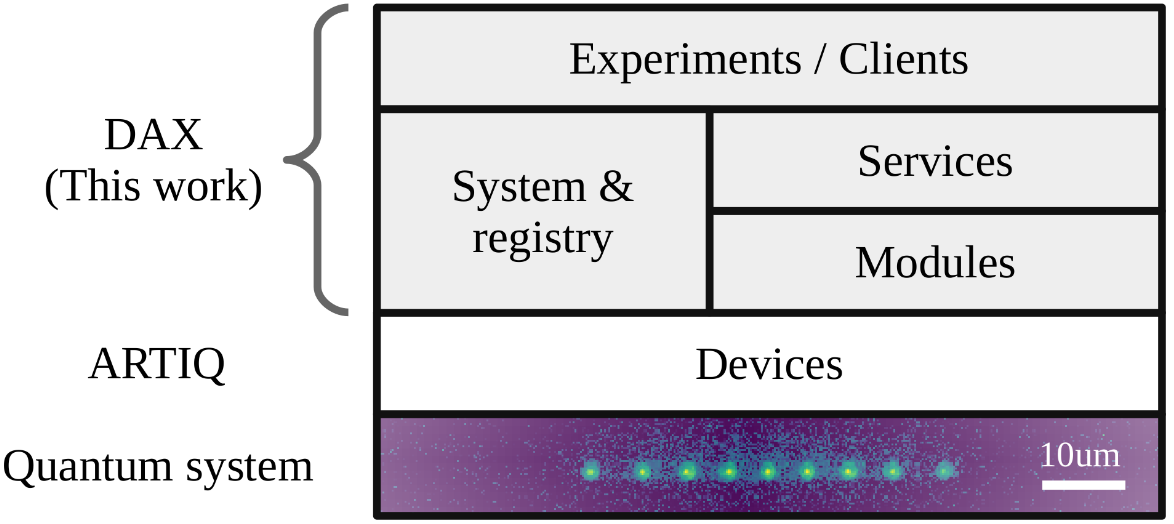
\includegraphics[width=.8\textwidth]{overivew.png}
  \end{figure}
\end{frame}
\begin{frame}{Experiment}
  \begin{figure}
    \subfigure{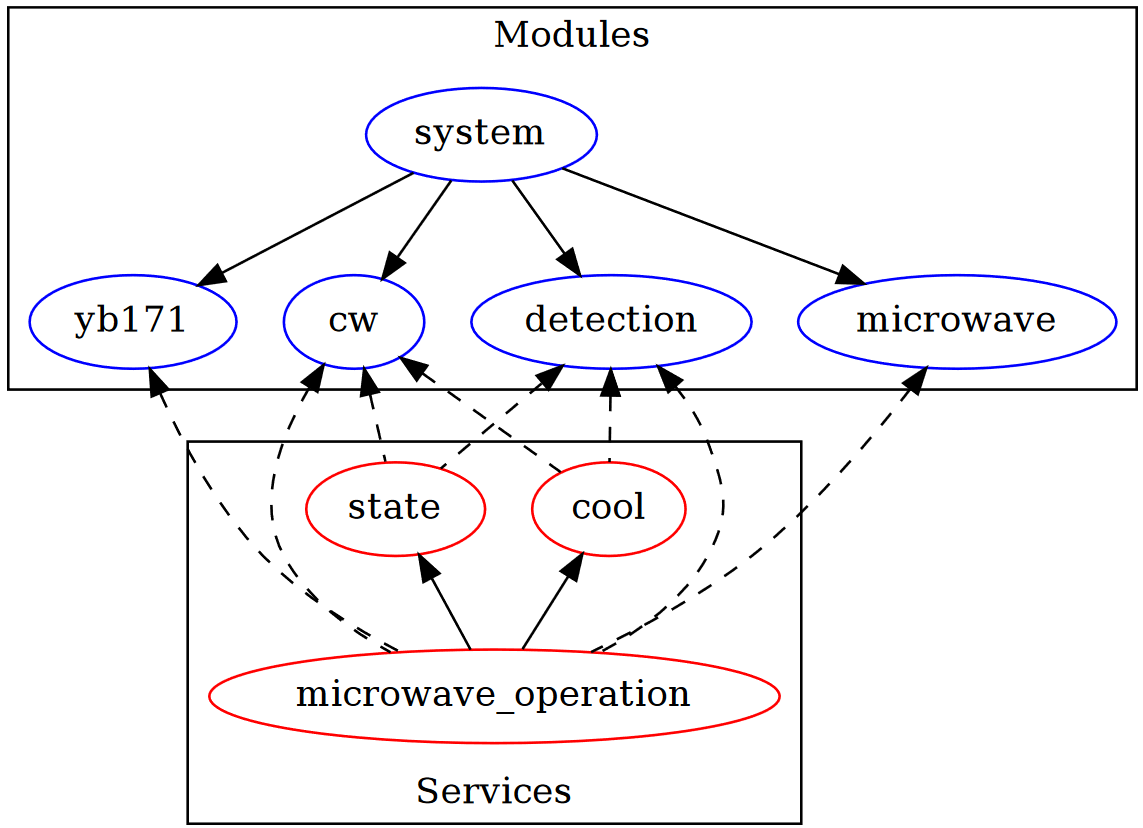
\includegraphics[width=.4\textwidth]{STAQ.png}\caption{STAQ }}
    \subfigure{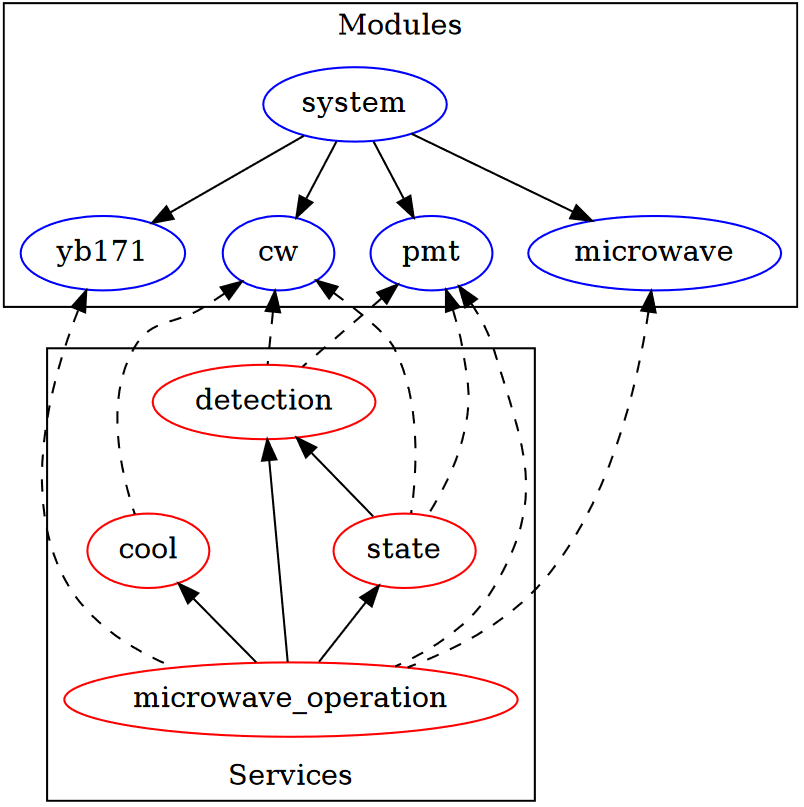
\includegraphics[width=.4\textwidth]{RC.png}\caption{RC }}
  \end{figure}
\end{frame}


\begin{frame}{Code Reuse Analysis}
  \begin{itemize}
  \item 49-91\% code reuse across two different systems
  \item Portable modules/services, interfaces, clients key enablers
  \end{itemize}
  \end{frame}
  
  \begin{frame}{Code Reuse Analysis}
    \begin{figure}
      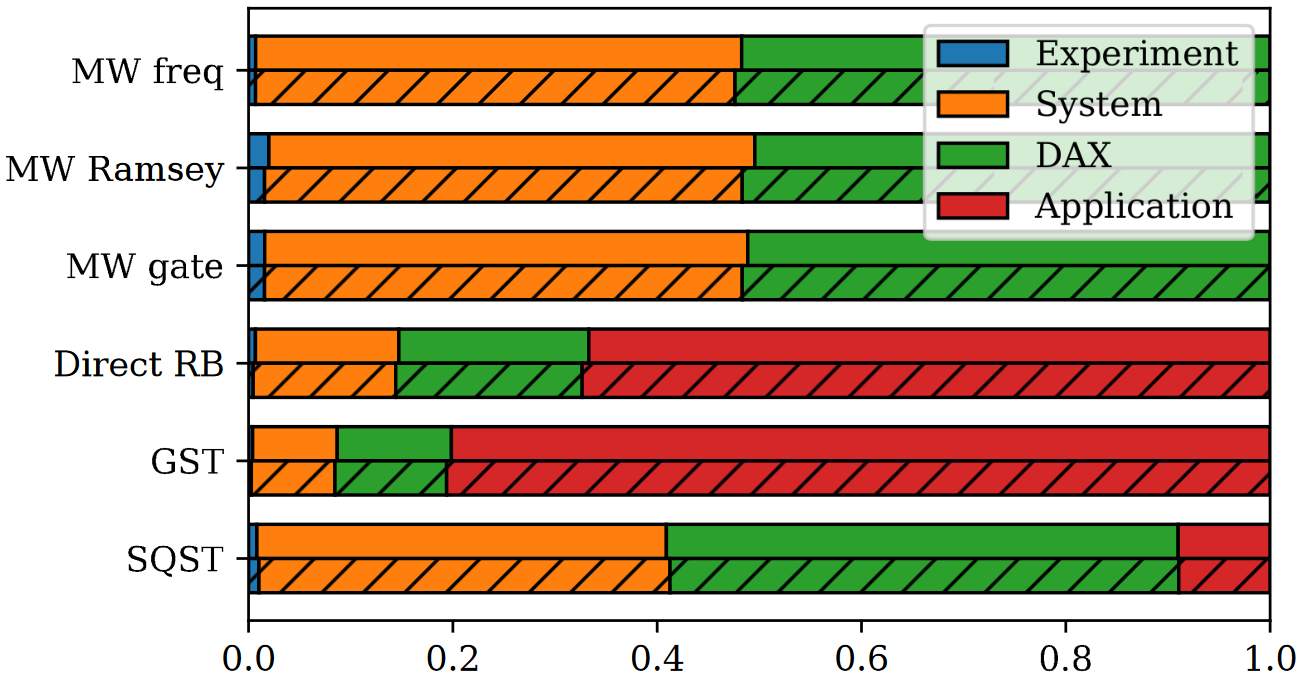
\includegraphics[width=.8\textwidth]{fig6.png}
    \end{figure}
  \end{frame}
  \begin{frame}{Code Reuse Analysis}
    \begin{figure}
      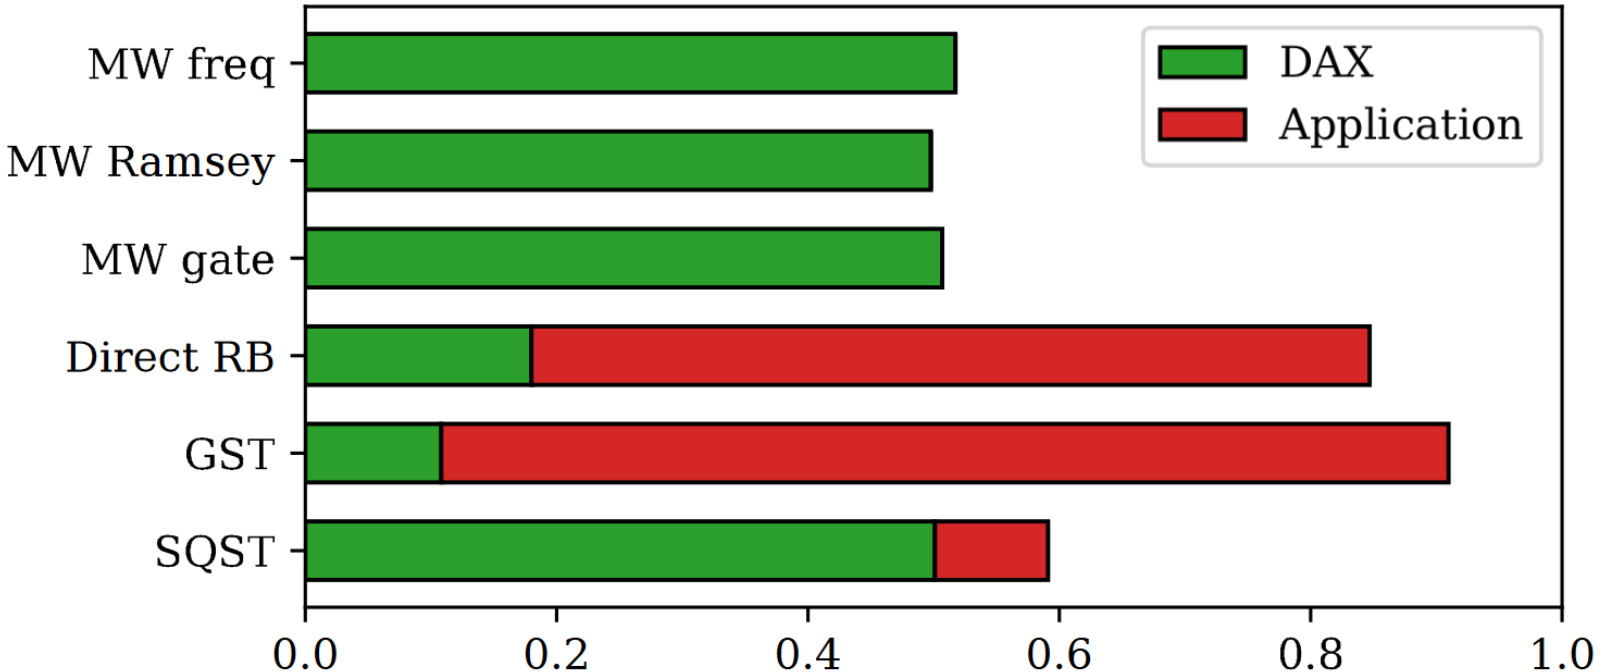
\includegraphics[width=.8\textwidth]{fig7.png}
    \end{figure}
  \end{frame}
\begin{frame}{Performance Evaluation}
\begin{itemize}
\item 63\% lower execution overhead vs non-modular code
\item Similar binary size
\item Fine-grained timing management and data offloading
\end{itemize}
\end{frame}
\begin{frame}
  \begin{figure}
    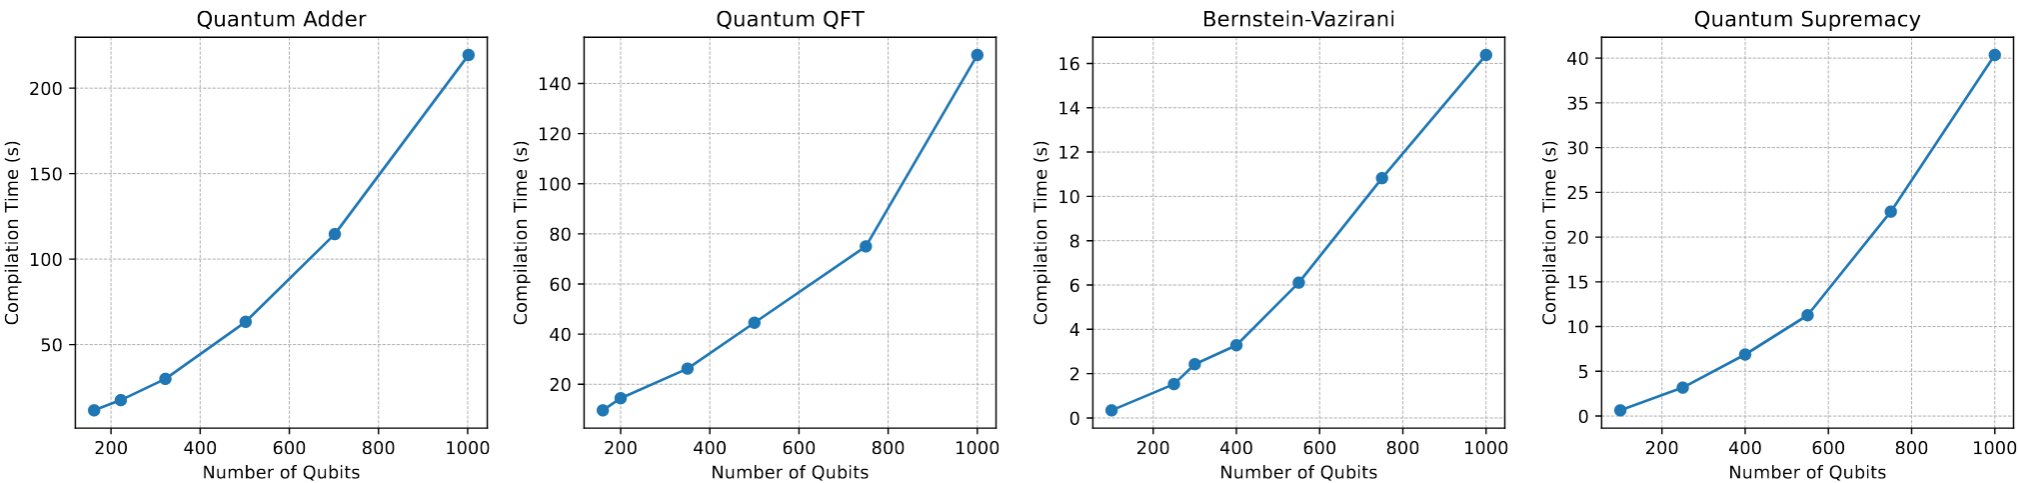
\includegraphics[width=.8\textwidth]{time.png}
  \end{figure}
\end{frame}

\begin{frame}{Conclusion}
\begin{itemize}
\item Modular architecture enables portable quantum control software
\item Reduces development overhead as hardware evolves
\item Important step towards scalable quantum systems
\end{itemize}

\end{frame}

\end{document}